\documentclass{bioinfo}
\copyrightyear{2015} \pubyear{2015}

\access{Advance Access Publication Date: Day Month Year}
\appnotes{Manuscript Category}

\usepackage{fancybox}
%\usepackage{enumitem}

%% diagonal line in a cell table
\usepackage{slashbox}

%\setcounter{secnumdepth}{6}

\usepackage{multirow} 
\usepackage[table]{xcolor}
\definecolor{lightgray}{gray}{0.9}

%strike-out words
\usepackage{soul}

\usepackage{hyperref}
\usepackage{xr}
\externaldocument{HPOSuppl}


\newcommand{\inda}{\phantom{1}\hspace{3mm}}
\newcommand{\indb}{\phantom{1}\hspace{8.5mm}}
\newcommand{\indc}{\phantom{1}\hspace{12mm}}
\newcommand{\indd}{\phantom{1}\hspace{16mm}}
\newcommand{\inde}{\phantom{1}\hspace{20mm}}
\newcommand{\indf}{\phantom{1}\hspace{24mm}}
\newcommand{\indg}{\phantom{1}\hspace{28mm}}
\newcommand{\indh}{\phantom{1}\hspace{32mm}}
\newcommand{\bs}{\boldsymbol{s}}

\newcommand{\by}{\boldsymbol{y}}
\newcommand{\bt}{\boldsymbol{t}}
\newcommand{\bP}{\boldsymbol{P}}
\newcommand{\bI}{\boldsymbol{I}}

\newcommand{\htd}{{\em HTD}}

\newcommand{\tpr}{{\em TPR}}

\newtheorem{theorem}{Theorem}
\newtheorem{corollary}{Corollary}
%\newproof{pf}{Proof}

\begin{document}
\firstpage{1}

\subtitle{Subject Section}

% A hierarchical ensemble approach for predicting genes associated to abnormal human phenotypes.

% Prediction of genes associated to abnormal human phenotypes through hierarchical ensemble methods.

\title[A hierarchical ensemble for HPO term prediction]{A hierarchical ensemble approach for predicting genes associated to abnormal human phenotypes}
\author[Sample \textit{et~al}.]{Marco Notaro\,$^{\text{\sfb 1}}$, Peter N. Robinson\,$^{\text{\sfb 2,3,4,5}}$ and Giorgio Valentini\,$^{\text{\sfb 1,}*}$}
\address{$^{\text{\sf 1}}$Anacleto Lab - Dipartimento di Informatica, Universit\'a degli Studi di Milano, Via Comelico 39, 20135 Milano, Italy \\
$^{\text{\sf 2}}$Institute for Medical and Human Genetics, Charite-Universitatsmedizin Berlin, Augustenburger Platz 1, 13353 Berlin, Germany\\
$^{\text{\sf 3}}$Max Planck Institute for Molecular Genetics, Ihnestrasse 63-73, 14195 Berlin, Germany\\
$^{\text{\sf 4}}$The Jackson Laboratory for Genomic Medicine, 10 Discovery Drive. Farmington, CT 06032, USA\\
$^{\text{\sf 5}}$Institute for Systems Genomics, University of Connecticut, Farmington, CT 06032, USA
}



\corresp{$^\ast$To whom correspondence should be addressed.}

\history{Received on XXXXX; revised on XXXXX; accepted on XXXXX}

\editor{Associate Editor: XXXXXXX}


\abstract{\textbf{Motivation:} \\
\textbf{Results:} \\
\textbf{Contact:} \href{name@bio.com}{name@bio.com}\\
\textbf{Supplementary information:} Supplementary data are available at \textit{Bioinformatics}
online.}

\maketitle

%%%%%%%%%%%%%%%%%%%%%%%%%%%%%%%%%%%5
\section{Introduction}
%Ontologies are computational representation of knowledge domains based upon controlled and standardized vocabularies 
%describing entities and semantic relationships between them. The Human Phenotype Ontology (HPO) aims at providing a standardized of the abnormalities associated with human diseases (each %represented by an HPO term) and the semantic relationship between them~\citep{Kohler14b}. More precisely, all the terms in HPO are structured according to a DAG and all the relationship are{\it is-a} (i.e. class-subclass relationships) and {\it transitive} (i.e. all relationships are inherited up to the root).\\
 
% - Introduction to HPO and its importance for human diseases
%% Nota: NON forzare gli a capo ccn \\
In medical contexts, the word ``{\it phenotype}'' is defined as a deviation from normal morphology, physiology, or behavior~\citep{deepheno}. 
The analysis of phenotype is essential for understanding the pathophysiology of cellular networks and plays a key role in medical research and in the mapping of disease genes~\citep{nick11}. The Human Phenotype Ontology project~\citep{nick8} aims at providing a standard categorization of the abnormalities associated to human diseases and the semantic relationships between them. It's worth noting that each HPO term does not represent a disease, but rather it denotes individual signs or symptoms or other clinical abnormalities that characterize a disease. Thus, one disease is characterized by one or more HPO terms and many HPO terms are associated with multiple distinct diseases. The HPO is currently developed using the medical literature, and OMIM~\citep{omim}, Orphanet~\citep{orphanet} and DECIPHER~\citep{decipher} databases, and contains approximately $11,000$ terms and over $115,000$ annotations to hereditary diseases. 
The HPO is structured according to a Direct Acyclic Graph (DAG), where more general terms are found on the top levels of hierarchy and the term specificity increases moving towards the lower levels of hierarchy, i.e. from root to leaves. The HPO is governed by {\it true-path-rule} (also known as {\it annotation propagation rule})~\citep{nick11}: if a gene is annotated with a given functional term, then it is annotated with all the ``parent'' classes, and with all its ancestors in a recursive way. On the contrary if a gene is not annotated to a class, it cannot be annotated to all its offspring. According to this rule, a positive prediction for a class and a negative prediction for its parent classes are not allowed, since this violates the inclusion relationship between them. 
% Therefore, a positive prediction for a given class implies positive predictions for all the ancestors of that class, and a negative prediction implies negative predictions for all its descendants, in order to avoid violating the {\it true path rule}.

% - Underlooking of the problem of the prediction of the associations genes - HPO term
While the problem of the prediction of the associations gene - disease has been widely investigated~\citep{Moreau12}, the related problem of the gene - HPO term prediction has been only considered  in a few studies~\citep{PHENO15}, despite no HPO term associations are known for most human genes, and the quickly growing application of the HPO to relevant medical problems~\citep{Zemojtel2014,Smedley16}.

% - Flat methods for HPO term prediction and their disadvantages
``Flat'' classification methods, that predict labels independently of each other, can in principle be applied to the prediction of gene - HPO terms associations~\citep{Wang13}, but they may introduce significant inconsistencies in the classification, since the predictions made are unaware of the hierarchical relationship between the different phenotypes, both in human and model organism~\citep{Musso14}.
For instance, if we adopt the HPO to catalogue human phenotypes and we try to predict HPO terms independently of each other, we could associate to a human gene the HPO term ``Hypoplasia of metatarsal bones'' but not the term ``Abnormalities of the metatarsal bones'', introducing thus an inconsistency since ``Hypoplasia of metatarsal bones'' is obviously a subclass of ``Abnormalities of the metatarsal bones''. Besides inconsistency, flat methods  may lose important a priori knowledge about the constraints of the hierarchical labeling that could enhance the accuracy of the predictions.

% - Structured output methods
To properly handle the hierarchical relationships between terms that characterize ontologies (including the HPO), we can apply two main classes of structured output methods, i.e. methods able to exploit in the learning process the hierarchical structure of terms~\citep{Vale14c}.
The first general approach is based on the kernelization of both the input and the output space through the introduction of techniques based on large margin methods for structured and interdependent output variables~\citep{Tsochantaridis05}. The second general approach is based on ensemble methods able to exploit the hierarchical relationship between classes~\citep{Silla11}. 

In the context of HPO, \citet{PHENO15} proposed a structured output method, based on a joint kernel constructed through the product of the input and the output kernel, and showed that the proposed approach  outperforms existing methods. 

% - Hirarchical ensemble methods
To our knowledge no methods based on hierarchical ensembles have been proposed in the context of structured output prediction of HPO terms associated with human genes.
Indeed most of the hierarchical ensemble methods proposed in literature are conceived for tree-structured taxonomies~\citep{Vale14c}, and the few ones specific for DAGs have been mainly applied to the prediction of the gene and protein functions~\citep{Obozinski08, Guan08}.

% - Advantages of our proposed methods
To fill this gap, we propose two distinct hierarchical ensemble methods (Section~\ref{hiermeth}) able to provide consistent predictions of HPO terms and to scale nicely both in terms of the complexity of the taxonomy and the cardinality of the examples.
The proposed approaches present several advantages with respect to structured output methods based on the joint kernelization of input and output:
\begin{enumerate}
\item Their computational complexity  is significantly lower, while the results are competitive with respect to state-of-the art methods
\item The methods are modular, in the sense that being ensembles, can be applied with different base learners, thus allowing to enhance the predictions of any flat learning method, used as base learner in the hierarchical ensemble. Indeed  hierarchical ensemble methods use as input the output of a generic flat method and are able to provide a structured prediction of the terms of the HPO according to the hierarchical relationships between terms.
\item These methods can be applied to improve the prediction of any base learner and are not constrained to apply a specific learning algorithm as it is done by kernelized method with structured output.
\item They are guaranteed to provide consistent predictions and can provide any structured prediction obeying the true path rule, differently from structured output kernelized methods that for computational complexity reasons are only able  to provide a predefined set of possible structured predictions~\citep{PHENO15}.
\end{enumerate}

% - Summary of next sections
In the next Section we describe the details of the proposed algorithm and we prove the consistency of the structured prediction of HPO terms.
Then in Section~\ref{sec:results-discussion} we present a genome-wide experimental comparison of our proposed hierarchical ensembles with state-of-the-art methods for HPO term prediction, and we show that hierarchical ensemble methods can accurately predict novel potential associations gene - HPO term.

[ {\bf Note}: We could try to predict potential novel associations for currently not annotated genes, but we need to perform the experiments ... Do you think that could be useful to provide such results?]


%\enlargethispage{12pt}
%%%%%%%%%%%%%%%%%%%%%%%%%%%%%%%%%%%%%%%
\begin{methods}

%%%%%%%%%%%%%%%%%%%%%%%%%%%%%%%%%%%%%
\section{Methods}
\label{hiermeth}

We present two algorithms, {\em Hierarchical Top-Down (HTD-DAG)} and {\em True Path Rule (TPR-DAG)} for {\em Directed Acyclic Graphs (DAG)}, specifically designed to exploit the DAG structure of the relationships between HPO terms to predict associations between genes and sets of HPO terms.

Both these hierarchical ensemble methods~\citep{Silla11} adopt a two-step learning strategy:
\begin{enumerate}
\item {\em Flat learning of the terms of the ontology}. In the first step each base classifier learns a specific class (HPO term). This yields a set of independent classification problems, where each base learning machine is trained to learn a specific class, independently of the other base learners.
\item {\em Hierarchical combination of the predictions}. In the second step the predictions provided by the trained classifiers are combined by considering the hierarchical relationships between the base classifiers modeled according to the hierarchy of the HPO.
\end{enumerate}
This ensemble approach is highly modular: in principle any learning algorithm can be used to train the classifiers in the first step, and in the second step the hierarchical relationships between the HPO terms are exploited to achieve the final ensemble predictions of the set of HPO terms associated to a specific gene.


%%%%%%%%%%%%%%%%%%%%%%%%%%%%%%%%%%%%%
\subsection{Basic notation and definitions}
Let $G = <V,E>$ a Directed Acyclic Graph (DAG) with vertices $V = \{1, 2, \ldots, |V| \}$ and edges $e=(i,j) \in E, i,j \in V$. $G$ represents the HPO taxonomy structured as a DAG, whose nodes $i \in V$ represent classes (terms) of the ontology and a directed edge $(i,j) \in E$ the hierarchical relationships between $i$ and $j$: $i$ is the parent term and $j$ is the child term. 
%We assume that does exist a unique root node $root(G)$ of the DAG; if there are multiple roots we can easily add a unique root node by simply adding an edge between the added root and the original multiple roots.

The set of children of a node $i$ is denoted by $child(i)$, the set of its parents by $par(i)$, the set of its ancestors by $anc(i)$ and the set of its descendants by $desc(i)$.

A ``flat multi-label scoring'' predictor  $f: X \rightarrow \mathbb{Y}$ provides a score $f(x) = \hat{\by},  \hat{\by} \in \mathbb{Y}=[0,1]^{|V|}$ for a given example $x \in X$, where $X$ is a suitable input space for the predictor $f$. In other words a flat predictor provides a score $\hat{y}_i \in [0,1]$ for each node/class $i \in V$ of the DAG $G$:
\vspace*{-5pt}
\begin{equation}
\hat{\by} = < \hat{y}_1, \hat{y}_2, \ldots, \hat{y}_{|V|}>
\vspace*{-5pt}
\end{equation} 


We say that the multi-label scoring $\by$ is consistent if it obeys the {\em true path rule}:
\vspace*{-5pt}
\begin{equation} 
\by \; {\rm is \; consistent}  \iff \forall i \in V, j \in par(i) \Rightarrow y_j \geq y_i 
\label{eq:cont-true-path-rule}
\vspace*{-5pt}
\end{equation}
From eq.~\ref{eq:cont-true-path-rule} descends that if we predict that a protein is annotated with a given term $i$ then to provide consistent predictions the same protein must be annotated also with all the ancestor terms of $i$.

In real cases it is very unlikely that a flat multi-label scoring predictor  satisfies the true path rule, since by definition the predictions are performed without considering the hierarchy of the classes. 
Nevertheless, by adding a further label/score modification step that takes into account the hierarchy of the classes, we can modify the labeling or the scores of the flat predictors to obtain a hierarchical classifier that obeys the true path rule. 
More precisely, we can provide a function $h(f(x)): \mathbb{Y} \rightarrow \mathbb{Y}$ such that the {\em true path rule} (\ref{eq:cont-true-path-rule}) holds for all the predictions $h(f(x)) = \bar{\by}$:
\vspace*{-5pt}
\begin{equation} 
 \forall i \in V, j \in par(i) \Rightarrow \bar{y}_j \geq \bar{y}_i 
\label{eq:vlid-hier-corr}
\vspace*{-0pt}
\end{equation}


%%%%%%%%%%%%%%%%%%%%%%%%%%%%%%%%%%%%%%%%%%%%%%%%%%%%%%%%%%%%%%%%%%%%%%%%
\subsection{Flat learning of the terms of the ontology}
At first the algorithm adopts  a flat ensemble learning strategy by which each term $i \in V$ of the HPO is independently learned through a term specific predictor $f_i : X \rightarrow [0,1]$. 
Accordingly, the output of the flat classifier $f:X \rightarrow  \mathbb{Y}$ on the instance $x \in X$ is $f(x) = \hat{\by}$:
\vspace*{-10pt}
\begin{equation}
f(x) = <f_1(x),\ f_2(x),\ \ldots,\ f_{|V|}(x)> =  <\hat{y}_1,\hat{y}_2,\ \ldots,\ \hat{y}_{|V|}> 
\vspace*{-5pt}
\end{equation}
%In other words a specific classifier $f_i$ is associated to each class $i$ in order to provide a flat evaluation of the membership of a specific example $x \in X$ to the class $i$. 
To this end any supervised or semi-supervised base predictor can be used, including also flat  binary classifiers, even if flat predictors $f_i$ estimating a score or a probability that gene $x$ belongs to a HPO term $i$  are better suited to this task.
Note that the training of per-class predictors $f_1,\ f_2,\ \ldots, f_{|V|}$ can be performed in parallel, and it is easy to achieve a linear speed-up in the number of the available processors by adopting simple parallel computational techniques. 
% Although at this step multi-task learning methods can also be applied to exploit the commonalities between related tasks~\cite{Caruana97}, in this work we did not adopt multi-task classifiers since we are mainly interested in developing hierarchical methods applicable as a next step to provide consistent predictions and to enhance the results of a generic flat method. 

%%%%%%%%%%%%%%%%%%%%%%%%%%%%%%%%%%%%%%%%%%%%%%%%%%%%%%%%%%%%%%%%%%%%%%%%
\subsection{The Hierarchical Top-Down (HTD) algorithm }
\label{subsec:HTD}
The main idea behind the Hierarchical top-down algorithm {\em (HTD-DAG)} consists in  modifying the predictions of each base learners from "top to bottom", i.e. from the least  to the most specific terms by exploiting at each  step the predictions provided by the less specific predictors, e.g. predictors associated to parent HPO terms. This is performed in a recursive way by transmitting the predictions from each node to the their children, and from the children to the children of the children through a propagation of the information towards the descendants of each node of the ontology. For instance in Fig.~\ref{fig:info-flow}a the information can flow along the path traversing nodes $1, 5, 6, 7$ or $1, 3, 7$ (numbers represent different HPO terms), and a prediction for e.g. the node $5$ depends on the predictions performed by the base learners for the parent nodes $4, 1$ and $3$. This operating mode of the ensemble is performed neatly from the top to the bottom nodes (Fig.~\ref{fig:info-flow}a).

%%%%%%%%%%%%%%%%%%%%%%%%%%%%%%%%%%%
\begin{figure}[!h]
%\vskip -0.1in
\centering
\begin{tabular}{cc}	
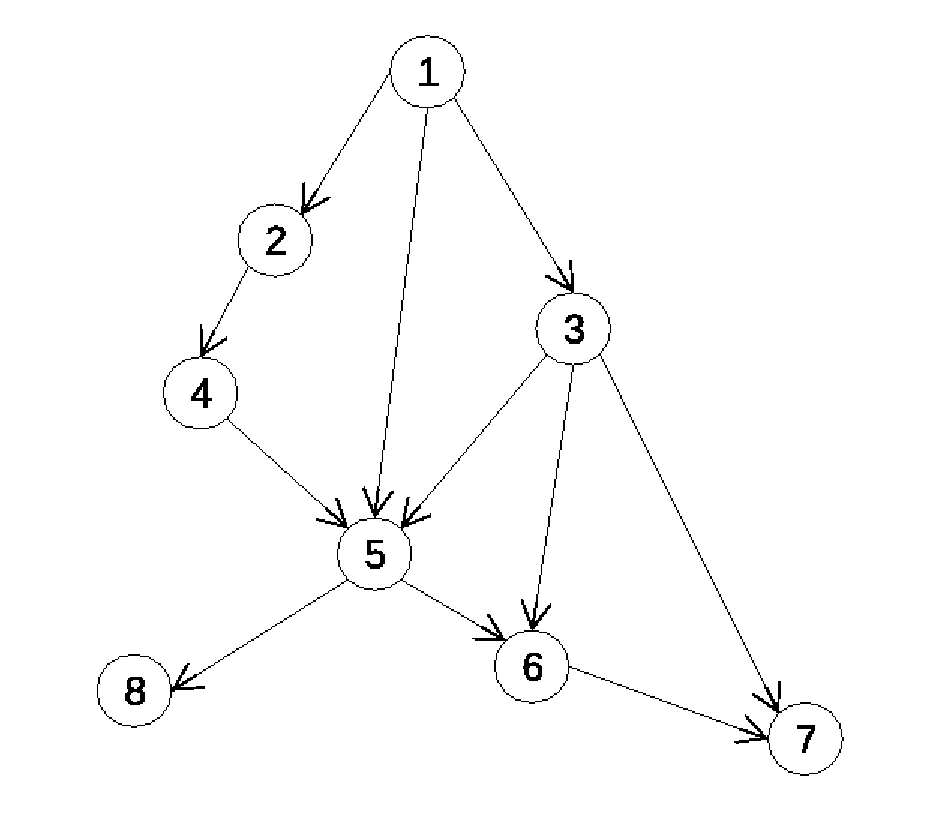
\includegraphics[width=4.0cm]{fig/top-down-flow.eps} &
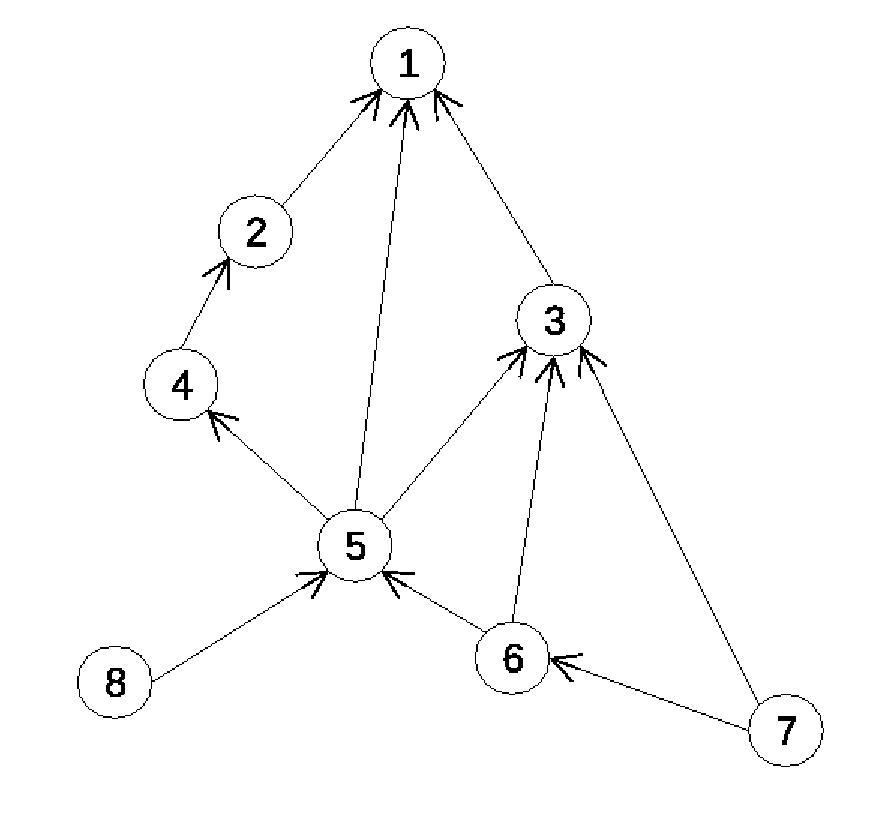
\includegraphics[width=4.0cm]{fig/bottom-up-flow.eps} \\
(a) & (b)\\ 
\end{tabular}
\vskip -0.1in
\caption{{\bf Flow of information in hierarchical ensembles.} (a) Top-down flow (b) Bottom-up flow. See text for more explanations.}
\label{fig:info-flow}
\vskip -0.1in
\end{figure}
%%%%%%%%%%%%%%%%%%%%%%%%%%%%%%%%%

More precisely, the  {\em HTD-DAG} algorithm modifies the flat scores according to the hierarchy of a DAG through a unique run across the nodes of the graph. For a given example $x \in X$, the flat predictions $f(x) = \hat{\by}$ are hierarchically corrected to $\bar{\by}$, by per-level visiting the nodes of the DAG from top to bottom, according to the following simple rule:
\begin{equation}
\bar{y}_i := \left\{
                 \begin{array}{lll}
				   \hat{y}_i  & {\rm if} \quad i \in root(G) \\
                   \min_{j \in par(i)} \bar{y}_j & {\rm if} \quad \min_{j \in par(i)} \bar{y}_j < \hat{y}_i \\
                   \hat{y}_i & {\rm otherwise}
                 \end{array}
                \right.
\label{eq:HTD} 
\end{equation}
The node levels correspond to their maximum path length from the root. 
If $p(r,i)$ represents a path from the root node $r$ and a node $i \in V$, $l \left(p(r,i)\right)$  the length of $p(r,i)$, $\mathcal L = \{0, 1, \ldots, \xi \}$ the set of observed levels, with $\xi$  the maximum node level, then $\psi: V \longrightarrow \mathcal L$ is a level function which assigns each node $i\in V$ to its level $\psi(i)$:
\vspace*{-5pt}
\begin{equation}
\psi(i) = \max_{p(r,i)}\ l \left(p(r,i)\right)
\label{eq:psi}
\vspace*{-5pt}
\end{equation}
Nodes $ \{i | \psi(i) = 0 \}$ correspond to the root nodes, $ \{i | \psi(i) = 1 \}$ is the set of nodes  with a maximum path length from the root (distance) equal to $1$, and $ \{i | \psi(i) = \xi \}$ are nodes that lie at a maximum distance $\xi$ from the root.


%%%%%%%%%%%%%%%%%%%%%%%%%%%%%%%%%%%%%%%%%%%%%%%%%%%%%%%%%%%%%%
%%%%%%%%%%%%%%%%%%%%%%%%%%%%%%%%%%%%%%%%%%%%%%%%%%%%%%%%%%%
\begin{figure}[!hb]
\begin{center}
\cornersize*{8pt}
\ovalbox{
\begin{minipage}{0.40\textwidth}
\caption{\bf{The Hierarchical Top-Down algorithm for DAGs (HTD-DAG)}}
\label{fig-HTD}

\noindent
{\tt Input}:\\
- $G = <V,E>$\\
%%- $V = \{1, 2, \ldots, |V| \}$\\
- $\hat{\by} = < \hat{y}_1, \hat{y}_2, \ldots, \hat{y}_{|V|}>$ (flat predictions) \\
\noindent
{\tt begin algorithm}\\
01:  \inda   A. $dist := $ ComputeMaxDist $(G, root(G))$ \\
02:  \inda   B. Per-level top-down visit of $G$:\\
03:    \indb $\bar{y}_{root(G)} := \hat{y}_{root(G)}$\\
04:    \indb {\tt for each} $d$ {\tt from} $1$ {\tt to} $\xi$ {\tt do}\\
05:      \indc  $N_d := \{ i | dist(i) = d \}$\\
06:      \indc  {\tt for each} $i \in N_d$ {\tt do}\\
07:          \indd  $x := \min_{j \in par(i)} \bar{y}_j$\\
08:          \indd  {\tt if} $(x < \hat{y}_i)$\\
09:             \inde  $\bar{y}_i := x$\\
10:          \indd  {\tt else}\\
11:             \inde  $\bar{y}_i := \hat{y}_i$\\
12:      \indc  {\tt end for}\\
13:    \indb {\tt end for}\\
{\tt end algorithm}\\
\noindent
{\tt Output}:\\
- $\bar{\by} = < \bar{y}_1, \bar{y}_2, \ldots, \bar{y}_{|V|}>$\\
\end{minipage}
}
\end{center}
\end{figure}


%%%%%%%%%%%%%%%%%%%%%%%%%%%%%%%%%%%%%%
%\subsection{Computing node levels in DAG}\label{sub:maxDist}

Fig.~\ref{fig-HTD} shows the pseudo code of the second step of {\em HTD-DAG} algorithm, by which the flat predictions $\hat{\by}$ computed in the first step are combined and updated according to top-down per-level traversal of the DAG.

The block A of the algorithm (row  $1$) computes the maximum distance of each node from the root; to this end the classical Bellman-Ford algorithm or the methods based on the Topological Sorting algorithm can be applied~\cite{Cormen09}.

The block B of the algorithm implements a per-level top-down visit of the graph (rows $2-13$). 
Starting from the children of the root (level $1$) for each level of the graph the nodes are processed and the hierarchical top-down correction of the flat predictions $\hat{y}_i$, $i \in \{1, \ldots, |V| \}$ is performed according to~(\ref{eq:HTD}) thus obtaining the {\em HTD-DAG} ensemble prediction  $\bar{y}_i$.
More precisely, the nested loops starting respectively at line $04$ and $06$ ensure that nodes are processed by level in an increasing order. Lines $07$--$11$, which implement (\ref{eq:HTD}), perform the hierarchical correction of the flat predictions $\hat{y}_i$, $i \in \{1, \ldots, |V| \}$.
The algorithm ends when, at the last iteration of the external loop (lines $04$--$13$),  nodes at distance $\xi$ from the root are processed, and provides as output the corrected predictions $\bar{\by}$.

The complexity of block $A$ is $\mathcal{O}(|V| + |E|)$ (if the Topological Sort algorithm is used to implement {\em ComputeMaxDist}),
while it is easy to see that the complexity of block $B$ (rows $3-13$) is $\mathcal{O}(|V|+|E|)$.
Hence the overall complexity of the top-down step of {\em HTD-DAG} is $\mathcal{O}(|V|+|E|))$, that is linear in the number of vertices for sparse graphs.


%%%%%%%%%%%%%%%%%%%%%%%%%%%%%%%%%%%%%%%%%%%%%
\subsection{Hierarchical True Path Rule algorithm for DAGs (TPR-DAG)}
\label{subsec:TPR}
The {\em HTD} algorithm takes only into account the predictions of the parent and recursively of the ancestor nodes. By considering the opposite flow of information "from bottom to top", we can construct the prediction of the ensemble by using the predictions made by the children  nodes and recursively by the descendant more specific nodes. For instance in Fig.~\ref{fig:info-flow}b) a possible flow of information could be along the path $8, 5, 4, 2, 1$ or $7, 6, 5, 1$, and the prediction of the ensemble for e.g. node $3$ depends on children nodes $5, 6$ and $7$. The proposed True Path Rule for DAG {\em TPR-DAG} adopts this bottom-up flow of information, to take into account the predictions of the most specific HPO terms, but also the opposite flow from top to bottom to consider the predictions of the most specific terms.
This second algorithm can be considered a DAG extension of the {\em TPR} algorithm, originally proposed for tree-structured taxonomies~\citep{Vale11a}.
The main difference with respect to the original tree-version consists in the fact that the per-level traversal of the DAG is now performed through two completely distinct steps: a bottom-up per level visit of the graph followed by a top-down visit, while in the original tree-version the per-level traversal is performed in an ``interleaved'' fashion (that is the bottom-up and top-down traversal are alternated at each level~\cite{Vale11a}). 
In the DAG version the separation of the bottom-up and top-down steps is necessary to assure the true path rule consistency of the predictions (see Section~\ref{sub:consistency} for details).


%%%%%%%%%%%%%%%%%%%%%%%%%%%%%%%%%%%%%%%%%%%%%%%%%%%%%%%%%%%
\begin{figure}[!h]
\begin{center}
\cornersize*{8pt}
\ovalbox{
\begin{minipage}{0.40\textwidth}
\caption{\bf{Hierarchical True Path Rule algorithm for DAGs (TPR-DAG)}}
\label{fig-TPR}
\noindent
{\tt Input}:\\
- $G = <V,E>$\\
- $V = \{1, 2, \ldots, |V| \}$\\
- $\hat{\by} = < \hat{y}_1, \hat{y}_2, \ldots, \hat{y}_{|V|}>, \quad  \hat{y}_i \in [0,1]$\\
%- $\bt = < t_1, t_2, \ldots, t_{|V|}>, \quad  t_i \in [0,1]$\\
\noindent
{\tt begin algorithm}\\
01:  \inda   A. Compute $\forall i \in V$ the max distance from $root(G)$:\\
02:    \indb $E' := \{e' | e \in E, \, e' = - e \}$\\
03:    \indb $G' := < V, E' >$\\
04:    \indb $dist := $ Bellman.Ford$(G', root(G'))$ \\
05:  \inda   B. Per-level bottom-up visit of $G$:\\ 
06:    \indb {\tt for each} $d$ {\tt from} $\max(dist)$  {\tt to} $0$ {\tt do}\\
07:      \indc  $N_d := \{ i | dist(i) = d \}$\\
08:      \indc  {\tt for each} $i \in N_d$ {\tt do}\\
09:          \indd  Select the set $\phi_i$ of ``positive'' children \\
10:          \indd  $\bar{y}_i := \frac{1}{1 + |\phi_i|} (\hat{y}_i + \sum_{j \in \phi_i} \bar{y}_j)$ \\
11:      \indc  {\tt end for}\\
12:    \indb {\tt end for}\\
13:  \inda   C. Per-level top-down visit of $G$:\\
14:    \indb $\hat{\by} := \bar{\by}$\\
15:    \indb {\tt for each} $d$ {\tt from} $1$ {\tt to} $\max(dist)$ {\tt do}\\
16:      \indc  $N_d := \{ i | dist(i) = d \}$\\
17:      \indc  {\tt for each} $i \in N_d$ {\tt do}\\
18:          \indd  $x := \min_{j \in par(i)} \bar{y}_j$\\
19:          \indd  {\tt if} $(x < \hat{y}_i)$\\
20:             \inde  $\bar{y}_i := x$\\
21:          \indd  {\tt else}\\
22:             \inde  $\bar{y}_i := \hat{y}_i$\\
23:      \indc  {\tt end for}\\
24:    \indb {\tt end for}\\
{\tt end algorithm}\\
\noindent
{\tt Output}:\\
- $\bar{\by} = < \bar{y}_1, \bar{y}_2, \ldots, \bar{y}_{|V|}>$\\
\end{minipage}
}
\end{center}
\end{figure}


The other main difference consists in the way the levels are computed: in this new DAG version the levels are constructed according to the maximum distance from the root, since this guarantees that in the top-down step all the ancestor nodes have been processed before their descendants, thus assuring the true path rule consistency of the predictions. 

%%%%%%%%%%%%%%%%%%%%%%%%%%%%%%%%%%%%%%%%%%%%%
%\subsubsection{The basic {\em TPR} algorithm for DAGs}
%\label{subsubsec:TPR-basic}

Similarly to the tree-based version the {\em TPR} algorithm, the basic {\em TPR-DAG} adopts a per-level bottom-up traversal of the DAG, starting from the nodes most distant (in the sense of the maximum distance) from the root to correct the flat predictions $\hat{y}_i$:

\begin{equation}  
\bar{y}_i := \frac{1}{1 + |\phi_i|} (\hat{y}_i + \sum_{j \in \phi_i} \bar{y}_j)
\label{eq:TPR}
\end{equation}
where $\phi_i$ are the ``positive'' children of $i$.

Here we consider only positive predictions of the children to obey the true path rule. Indeed, according to this rule, we may have a gene annotated to a term $t$, but not annotated to a terms $s \in child(t)$. Hence if we have a negative prediction for the terms $s$ it is not meaningful to use this prediction to predict the term $t$.
Different strategies to select the  ``positive'' children $\phi_i$ can be applied, according to the usage of a specific threshold to separate positive form negative examples:

\begin{enumerate}
\item {\em Constant Threshold (CT) strategy.} 
For each node the same threshold $\bar{t}$ is a priori selected: $t_j = \bar{t}, \quad \forall j \in V$.
In this case $\forall i \in V$ we have:
\begin{equation} 
\phi_i := \{ j \in child(i) | \bar{y}_j > \bar{t} \}
\label{eq:phi-constant}
\end{equation}
For instance if the predictions represent probabilities it could be meaningful to a priori select $\bar{t} = 0.5$.
\item {\em Adaptive Threshold (AT) strategy.}
The threshold is selected to maximize some performance metric $\mathcal{M}$ estimated on the training data, e.g. the F-score or the AUC. In other words the threshold is selected to maximize some measure of accuracy of the predictions $\mathcal{M}(j,t)$  on the training data for the class $j$ with respect to the threshold $t$. The corresponding set of positives  $\forall i \in V$ is:
\begin{equation} 
\phi_i := \{ j \in child(i) | \bar{y}_j > t_j^*,  t_j^* = \arg \max_{t} \mathcal{M}(j,t) \}
\label{eq:phi-adaptive}
\end{equation} 
For instance $t_j^*$ can be selected from a set of $t \in (0,1)$ through internal cross-validation techniques.
%\item $t_j$ is selected on the basis of the distribution of the positive examples available for the training set (e.g. $t_j$ could correspond to the $k^{th}$ percentile of the positive examples distribution).
\item {\em Threshold Free (TF) strategy.}
A different solution, that does not require an a priori or an experimentally selected threshold could consists in choosing those children that can increment the score of the node $i$ (that is  positive nodes are those that achieve a higher score than that of their parent):
\begin{equation} 
\phi_i := \{ j \in child(i) | \bar{y}_j > \hat{y}_i \}
\label{eq:phi-free}
\end{equation}
\end{enumerate}
According to the above positives selection strategies we can derive three different algorithmic variants of the basic {\em TPR}:
\begin{enumerate}
\item {\em TPR-CT}: {\em TPR} with constant threshold, corresponding to the above positives selection strategy a)
\item {\em TPR-AT}: {\em TPR} with adaptive thresholds, corresponding to the selection strategy b)
\item {\em TPR-TF}: {\em TPR} threshold-free, corresponding to the selection strategy c)
\end{enumerate}

With all the variants of the basic {\em TPR}, predictions are bottom-up propagated, thus moving positive predictions towards the parents and recursively towards the ancestors of each node.


Fig.~\ref{fig-TPR} shows the high-level pseudo-code of the {\em TPR-DAG} algorithm.
The first four rows compute the maximum distance of each node from the root, using the Bellman-Ford algorithm.
The block $B$ (rows 5-12) performs a bottom-up visit of the graph and updates the predictions $\bar{y}_i$ of the {\em TPR-DAG} ensemble according to eq.~\ref{eq:TPR} and one of the positives selection strategies described previously in this section.
Note that this step propagates the ``positive'' predictions from bottom to top of the DAG, but 
does not assure the true path rule consistency of the predictions.
This is accomplished by the third block (rows $13-24$) that simply executes a hierarchical top-down step, in the same way of the {\em HTD-DAG} algorithm.

The complexity of the {\em TPR-DAG} algorithm is quadratic in the number of nodes for the block $A$ (but can be  $\mathcal{O}(|V|+|E|)$ if the Topological Sort algorithm is used instead).
It is easy to see that the complexity is $\mathcal{O}(|V|)$ for both the $B$ and $C$ blocks when graphs are sparse.

A {\em TPR-DAG} variant similar to the weighted True Path Rule algorithms for tree-structured taxonomies~\cite{Vale12a} can be designed for DAGs.
The {\em TPR-W} can be obtained by substituting row $10$ of the {\em TPR-DAG} algorithm (Fig.~\ref{fig-TPR}) with the following line of pseudocode:
\begin{equation}
\bar{y}_i := w \hat{y}_i + \frac{(1 - w)}{|\phi_i|} \sum_{j \in \phi_i} \bar{y}_j
\label{eq:tpr-w}
\end{equation}
In this approach a weight $w \in [0,1]$ is added to balance between the contribution of the node $i$ and that of its ``positive'' children. If $w=1$ no weight is attributed to the children and the {\em TPR-DAG} reduces to the {\em HTD-DAG} algorithm, since in this way only the prediction for node $i$ is used in the bottom-up step of the algorithm.
If $w=0$ only the predictors associated to the children nodes "vote" to predict node $i$. In the intermediate cases for increasing values of $w$ we attribute more importance to the predictor for the node $i$ with respect to its children and of course we put more weights on children for decreasing values of $w$.

Other variants of the {\em TPR-DAG} algorithm can be designed by using at each step all the descendants of a given node instead of simply its children, or taking into account the accuracy of each base learner at each step of the weighted combination of the predictor (see Supplementary Information for more details).





%%%%%%%%%%%%%%%%%%%%%%%%%%%%%%%%%%%%%%%%%%%%%%%%%%%%%%%%%%%%%%%%%%%%%%%%%%%%%%%%%%%%%%%%%%
%%%%%%%%%%%%%%%%%%%%%%%%%%%%%%%%%%%%%%%%%%%%%%%%%%%%%%%%%%%%%%%%%%%%%%%%%%%%%%%%%%%%%%%%%%%%
\subsection{Consistency of the predictions}
\label{sub:consistency}
To obtain consistent predictions, we need to visit the hierarchy per level in the sense of the maximum and not of the minimum distance from the root.

Fig.~\ref{fig:max-dist-consistency} provides a simple example to show this fact. 
%%%%%%%%%%%%%%%%%%%%%%%%%%%%%%%%%%%%%%%%%%%%%%%%%%%%%%%%%%%
\begin{figure}[!htb]
\begin{center}
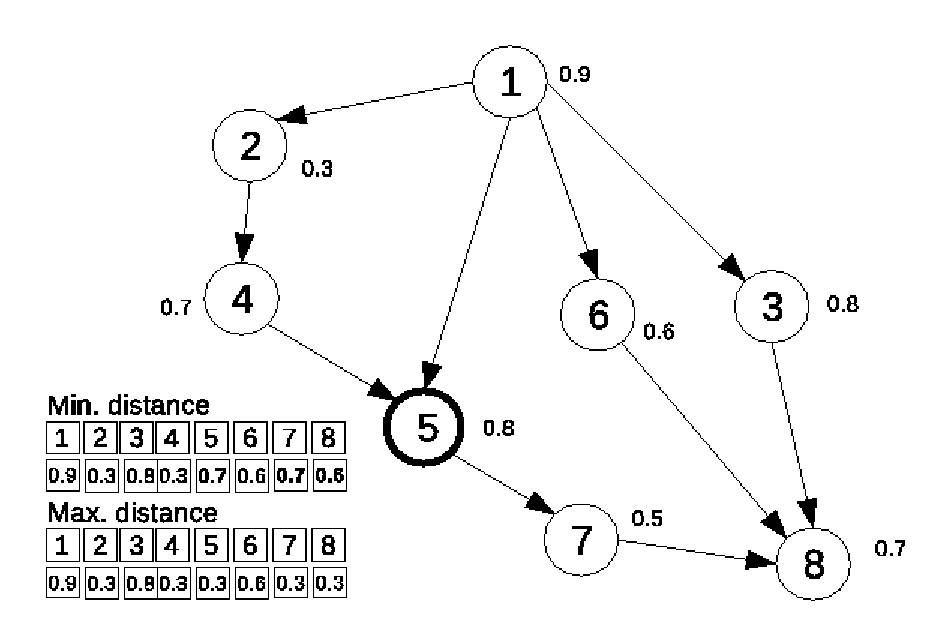
\includegraphics[scale=0.5]{fig/distTCS.eps} 
\caption{Levels defined in terms of the minimum distance from the root (node 1) lead to inconsistent predictions. The small numbers close to nodes correspond to the $\hat{y}_i$ scores of the flat predictions. The Hierarchical top-down scores obtained respectively by crossing the levels according to the minimum and the maximum distance from the root are shown in the bottom-left. Scores in boldface represent inconsistent predictions.}
\label{fig:max-dist-consistency}
\end{center}
\end{figure}
%%%%%%%%%%%%%%%%%%%%%%%%%%%%%
Indeed looking at the {\em HTD-DAG}  scores obtained respectively with the minimum and maximum distance from the root (bottom-left of Fig.~\ref{fig:max-dist-consistency}), we see that only the maximum distance preserves the consistency of the predictions.
For instance, focusing on node $5$, by traversing the DAG levels according to the minimum distance from the root, we have that the level of node $5$ is $1$ ($\psi^{min}(5)=1$) and in this case by applying the {\em HTD} rule (\ref{eq:HTD}) the flat score $\hat{y}_5 = 0.8$ is wrongly modified with the {\em HTD} ensemble score $\bar{y}_5 = 0.7$.
If we instead traverse the DAG levels according to the maximum distance from the root, we have $\psi^{max}(5)=3$ and the {\em HTD} ensemble score is correctly set to $\bar{y}_5 = 0.3$. In other words at the end of the {\em HTD}, by traversing the levels according to the minimum distance we have $\bar{y}_5 = 0.7 > \bar{y}_4 = 0.3$, that is a child note has a score larger than that of its parent, and the true path rule is not preserved. On the contrary by traversing the levels according to the maximum distance we achieve  $\bar{y}_5 = 0.3 \leq \bar{y}_4 = 0.3$ and the true path rule consistency is assured. 
This is due to the fact that by adopting the minimum distance when we visit node $5$, node $4$ has not just been visited, and hence the value $0.4$ has not been transmitted by node $2$ to node $4$; on the contrary if we visit the DAG according to the maximum distance all the ancestors of node $5$ (including node $4$) have just been visited and the score $0.4$ is correctly transmitted to node $5$ along the path $2 \rightarrow 4 \rightarrow 5$.

We proved the consistency of the predictions of both the {\em HTD-DAG} and {\em TPR-DAG} through the following theorems:
\begin{theorem} 
Given a DAG $G = <V,E>$, a level function $\psi$ that assigns to each node its maximum path length from the root and the set of {\em HTD-DAG} flat predictions $\hat{\by} = < \hat{y}_1, \hat{y}_2, \ldots, \hat{y}_{|V|}>$, the top-down hierarchical correction of the {\em HTD-DAG} algorithm assures that the set of ensemble predictions $\bar{\by} =< \bar{y}_1, \bar{y}_2, \ldots, \bar{y}_{|V|}>$ satisfies the following property: 
\[
\forall i \in V, \;  j \in par(i) \Rightarrow \bar{y}_j \geq \bar{y}_i
\]
\label{th:htd}
\end{theorem}
From Theorem~\ref{th:htd} it is easy to prove that the consistency of the predictions holds for all the ancestors of a given node $i \in V$. 
\begin{corollary}\label{cor:hier-consistency} Given a DAG $G = <V,E>$, the level function $\psi$ and the set of flat predictions $\hat{\by} = < \hat{y}_1, \hat{y}_2, \ldots, \hat{y}_{|V|}>$,  the {\em HTD-DAG} algorithm assures that for the set of ensemble predictions $\bar{\by} = < \bar{y}_1, \bar{y}_2, \ldots, \bar{y}_{|V|}>$ the following property holds: $\forall i \in V, \;  j \in anc(i) \Rightarrow \bar{y}_j \geq \bar{y}_i$.
\end{corollary}
Independently of the choice of the positive children (Section~\ref{subsec:TPR}), the following consistency theorem holds for {\em TPR-DAG}:
\begin{theorem} Given a DAG $G = <V,E>$, a set of flat predictions $\hat{\by} = < \hat{y}_1, \hat{y}_2, \ldots, \hat{y}_{|V|}>$ for each class associated to each node $i \in \{1, \ldots, |V| \}$,  the {\em TPR-DAG} algorithm assures that for the set of ensemble predictions $\bar{\by} = < \bar{y}_1, \bar{y}_2, \ldots, \bar{y}_{|V|}>$ the following property holds: $\forall i \in V, \;  j \in anc(i) \Rightarrow \bar{y}_j \geq \bar{y}_i$.
\end{theorem}
Finally a good property of {\em TPR-DAG} is that its sensitivity is always equal or better than that of the {\em HTD-DAG}:
\begin{theorem}
The {\em TPR-DAG} ensemble algorithm with ``positive'' children selected according to (\ref{eq:phi-free}) achieves always a sensitivity equal or higher than the {\em HTD-DAG} ensemble algorithm.
\end{theorem}
Unfortunately there is no guarantee that the precision of {\em TPR-DAG} is always larger or equal than that of the {\em HTD-DAG} algorithm.

All the proofs and details about the above theorems are available in the Supplementary Information.

\end{methods}



%%%%%%%%%%%%%%%%%%%%%%%%%%%%%%%%%%%%%%%%%%%%%%%%%%%%%%%%%%%%%%%%%%%%%%%%%%%%%%%%%%%%%%%%%%%%%%%%%%%%%%%%%%%%%%%%%%%%%%%%%%%%%%%
%%%%%%%%%%%%%%%%%%%%%%%%%%%%%%%%%%%%%%%%%%%%%%%%%%%%%%%%%%%%%%%%%%%%%%%%%%%%%%%%%%%%%%%%%%%%%%%%%%%%%%%%%%%%%%%%%%%%%%%%%%%%%%%

\section{Experimental results}
\label{sec:results-discussion}
We performed two different sets of experiments to compare our proposed hierarchical ensemble approach with state-of-the-art methods for the prediction of abnormal human phenotypes structured according to the HPO.
In the first set of experiments (Section~\ref{expI}) we compared \htd~and \tpr~ensembles with  state-of-the-art methods
using the same data and experimental set-up adopted by~\citet{PHENO15}.
In the second set of experiments (Section~\ref{expII}) we evaluated the ability of our proposed hierarchical ensemble methods to predict newly
annotated genes of the April 2016 HPO release, by using annotations of a previous release (January 2014).
 
%%% =============== EXP 1 =============== %%%
\subsection{Prediction of Human Phenotype Ontology terms}
\label{expI}
We compared the hierarchical ensemble methods for DAGs (\htd, Section~\ref{subsec:HTD}) and \tpr~and its variants, (Section~\ref{subsec:TPR}) against several state-of-the-art and baseline methods: 
\begin{itemize}
\item PHENOstruct, a state-of-the art joint-kernel structured support vector machine approach~\citep{PHENO15};
\item Clus-HMC-Ens, a state-of-the art Hierarchical Multilabel classification (HMC) based on decision tree ensemble~\citep{Schietgat10};
\item \textsl{SSVM} $\rightarrow$ {\em disease} $\rightarrow$ \textsl{HPO} {\em method}, an indirect two-step method that first predicts gene-disease associations and then maps them to HPO terms using the associations available on the HPO website~\citep{PHENO15};
\item {\em PhenoPPIOrth}, a computational tool that can predict a set of OMIM diseases for given human genes using protein-protein interaction and orthology data and then maps the predicted OMIM terms to HPO terms by direct mapping~\citep{Wang13}.
\item Probabilistic support vector machines (SVMs)~\citep{Pla99};
\item RANKS, a semi-supervised method base on kernelized score functions~\citep{Vale16a}, resulted one of the top-ranked methods in the recent CAFA2 challenge for HPO term prediction~\citep{Jiang16}.
\end{itemize}

We used both a semi-supervised  ({\em RANKS}~\citet{Vale16a}) and a supervised (Support Vector Machines -- SVM) machine learning method to implement the base learners of the proposed hierarchical ensemble methods (see Supplementary Information for more details).

We applied the same experimental set-up adopted by~\citet{PHENO15} to provide a fair comparison with previously proposed methods~\citep{Schietgat10, Wang13, PHENO15}. 

%In the next sections we describe the data used in our experiments (Section~\ref{dataset}), the experimental set-up and the performance metrics we used to evaluate the results (Section~\ref{eval}), the base learners used to train the hierarchical ensembles (Section~\ref{bl}), and finally in Section~\ref{res} we present and discuss the comparative experimental results.  

%%%%%%%%%%%%%%%%%%%%%%%%%%%%%%%%
\subsubsection{Data}
\label{dataset}
%The hierarchical ensemble methods proposed in section~\ref{hiermeth} require in input the molecular feature vectors (paragraph~\ref{net}), the graph representing the hierarchy of the classes and the annotation file, both described in paragraph~\ref{hpo}.

\paragraph{Data sources.}
\label{net} 
We used the same version of the the STRING (v. 9.1,~\citet{String91}) and BioGRID (v. 3.2.106,~\citet{biogrid13}) databases for a fair comparison with the results presented by~\citet{PHENO15}. More precisely we downloaded  physical and genetic experimental interactions relative to $4970$ proteins from \href{http://thebiogrid.org/}{BioGRID 3.2.106}, and the integrated  protein-protein interaction and functional association data for $18,172$ proteins from \href{http://string91.embl.de/}{STRING 9.1}. From the same STRING website we downloaded also the protein aliases file to map proteins to genes. 
%GV  Allora lo volgiamo specificare o no?
[NOTA: SPECIFICARE FRA QUALI IDENTIFICATORI HAI EFFETTUTATO IL MAPPING].

In STRING, each protein-protein interaction is annotated with a ``score'' ranging from $0$ to $1$ that indicates the confidence level of an interaction according to the available evidence and we used the full data available for {\em H. sapiens}.
%STRING evaluates an interaction being highly confident if the score is higher than $0.7$~\citep{String91_interaction}. Accordingly, in our experiments we constructed two distinct STRING functional bio-molecular interaction networks: one considering all the functional interactions and the other one considering only those interactions having a score $\geq 0.7$. In this work, we will refer to the former STRING network as {\it full} and to the latter as {\it filtered}. We did not remove singleton nodes from filtered network.

We used also $4$ different sources of gene annotation (GO BP, MF, CC and OMIM) to construct $4$ sets of similarity features between proteins through the classical Jaccard index, thus resulting in $4$ additional functional networks.
The resulting $n=6$ networks have been also integrated by averaging the  edge weights $w^d_{ij}$  between the genes $i$ and $j$, of each network $d \in \{1, n\}$, after normalizing their weights in the same range of values $w^d_{ij} \in [0,1]$ ({\it Unweighted Average} (UA) network integration,~\citet{Vale14e}):
%using a simple unweighted integration strategy, the {\it Unweighted Average} (UA) network integration~\citep{Vale14e}: we combined all the aforementioned $n=6$ gene networks by simply averaging the edge weights $w^d_{ij}$ of each network $d \in \{1, n\}$:
%In UA the weight of each edge of the combined networks is computed simply averaging across the available $n$ networks:
\begin{equation}
\bar{w}_{ij} = \frac{1}{n} \sum_{d = 1}^n w_{ij}^d
\label{eq:UA}
\end{equation}
More details about the data are available in the Supplementary Information.

\paragraph{HPO DAG and Annotations.}
\label{hpo}
Following the same experimental set-up of~\citet{PHENO15}, we considered separately the three main subontologies of the HPO (January 2014 release): {\it Organ Abnormality}, {\it Mode of Inheritance} and {\it Onset and Clinical Course}.
{\it Organ Abnormality} is the main ontology and includes terms related to clinical abnormalities. {\it  Mode of Inheritance} is a relatively small ontology and describes the inheritance pattern of the phenotypes. {\it Onset and Clinical Course} contains classes that describe typical modifiers of clinical symptoms, as the speed of progression, and the variability or the onset. 
For the sake of simplicity for the rest of the paper we refer to these subontologies respectively as {\it Organ}, {\it Inheritance} and {\it Onset}.
%Throughout this experimental part, we will refer to the {\it Organ Abnormality}, the {\it Mode of Inheritance} and the {\it Onset and Clinical Course} as respectively the {\it Organ }, {\it Inheritance} and {\it Onset} subontologies.
%the {\it Organ Abnormality}, the {\it Mode of Inheritance} and the {\it Onset and Clinical Course} will be referred as the {\it Organ subontology}, the {\it Inheritance subontology} and the {\it Onset subontology} respectively.
We pruned the HPO terms having less than 10 annotations in the January 2014 release. For the experiments we report the results obtained with STRING (the  most informative source of information, as reported by the analysis performed by~\citet{PHENO15}) and the UA integrated network.
The general characteristics of the resulting DAGs are reported in  Table~\ref{hpostat}.

%From the same HPO release we downloaded all the available gene-terms associations. Then we pruned the HPO terms having less than 10 annotations. 
%Since we considered two different gene-gene functional interaction (GGI) networks, i.e. the STRING and the UA integrated networks, we constructed two distinct HPO DAGs, each one related to the corresponding bio-molecular functional network. The number of terms (nodes) and the between-terms relationships (edges) of each HPO subontology are summarized in Table~\ref{hpostat}.


%% NOTA: togliere i colori dalla tabella
%% NOTA: STRING va indicata sempre in maiuscolo in tutto il paper.
%%%%%%%%%%%%%%%%%%%%%%%%%%%%%%%%
\begin{table}[!ht]
%\vskip -0.05in
%\rowcolors{1}{}{lightgray}
\centering
\caption{HPO DAG terms and between-terms relationship for each HPO subontology referred to the STRING and UA Integrated gene networks.}
\vskip 0.05in
\begin{tabular}{|c|c|c|c|} 
\hline
{\bf Subontology} & {\bf HPO Features} &  {\bf STRING Network} &  {\bf UA Network}\\ \hline
\cellcolor{white} & {\it nodes number } & 2134 & 2615\\ 
\multirow{-2}{*}{\cellcolor{white} Organ} & {\it edges number}  & 2154 & 2641\\ \hline
%
\cellcolor{white} & {\it nodes number} & 13 & 13\\ 
\multirow{-2}{*}{\cellcolor{white} Inheritance} & {\it edges number}  & 12 & 12 \\ \hline
%
\cellcolor{white} & {\it nodes number} & 23  & 24\\ 
\multirow{-2}{*}{\cellcolor{white} Onset} & {\it edges number}  & 22  & 23\\ \hline
\end{tabular} 
\vskip -0.1in
\label{hpostat}
\end{table}
%%%%%%%%%%%%%%%%%%%%%%%%%%%%%%%%%%


%%%%%%%%%%%%%%%%%%%%%%%%%%%%%%%%%%%%%%%%%%%%%%%%%%%%%%%%%%%%
\subsubsection{Experimental set-up and performance metrics}
\label{eval}
The generalization performance of the compared methods have been evaluated through a classical 5-fold cross-validation procedure, according to~\citet{PHENO15}.

%Since typically molecular biologists are interested in knowing both the set of genes associated with a certain HPO term and the phenotypic abnormalities associated with a particular human gene, we present the results using  respectively {\it term-centric} and {\it gene-centric} performance measures. 
%%  No queste defizinizioni sono sbagliate
%% {\it Protein-centric} measures average the performance across the examples, instead {\it term-centric} average the performance across terms~\citep{Radivojac2013}. More specifically,
%% as {\it term-centric} measure we used the $AUROC$ (Area Under the Receiver Operating Curve), computed by averaging AUC single values across HPO terms and several {\it protein-centric} measures as {\it F-max}, {\it Precision} and {\it Recall}.
We applied both {\it gene-centric} measures to provide metrics that depend on how much we can predict the HPO terms associated to each specific gene, and {\it term-centric} measures that focus on the accuracy achieved on each specific term of the ontology.
As {\it gene-centric} measure we used the hierarchical F-score, i.e. the harmonic mean of the hierarchical precision and recall computed separately for each specific gene. More precisely 
we applied the $F_{max}$ measure, i.e. the maximum hierarchical F-score achievable by ``a posteriori'' setting the optimal decision threshold (\citet{Jiang16}, see Supplementary Information for more details) 
%GV
% [NOTA: Marco, aggiungi le definizione formali di F-score gerarchico, ed F-max nelle Supplementary]. 
As {\it term-centric} measures we computed the classical Area Under the Receiving Operating Characteristic (AUROC). For both measures, by averaging across genes or terms, we may have an overall picture of the prediction performance of the methods.


%%%%%%%%%%%%%%%%%%%%%%%%%%%%%%%%%%%%%%%%%%%%%%%%%%%%%%%%%%%%
\subsubsection{Results and Discussion}
\label{res}


%% NOTA: usa in tutto il paper le macro \htd e \tpr per indicare i metodi. Non usare mai HTD e TPR
%% NOTA: qui non c'e' corrispondenza con i metodi indicati nella section~\ref{subsec:TPR}. 
%% Nota comunque che indicando i metodi se ne devono fornire le descrizioni, nel main paper o (meglio) nelle Supplementary.
%% Nel main paper verrano messi solo i risultati di TPR-w e per gli altri metodi si deve rimandare alle Supplementary, in cui verranno inseriti i risultati completi con tutte le varianti. 
We implemented five different \tpr~variants: {\em TPR-TF} (True Path Rule Threshold-Free), {\em TPR-CT} (True Path Rule with Constant Threshold), {\em TPR-W} (True Path Rule Weighted), {\em TPR-WT} (True Path Rule Weighted with Threshold) and  \textsl{TPR-D} (True Path Rule Descendants) (see Section~\ref{subsec:TPR} and Supplementary Information for more details).
[NOTA: Marco, controlla che le sigle e lo stile dei caratteri siano coerenti in TUTTO il paper e le Supplementary].

%% NOTA: Nella sezione Base Learner vengono desctirri due base learner, ma nei risultati viene riportato solo un risultato, senza perlatro specificare quale base learner e' stato usato. Quindi e' bene riportare entrambi i risultati nel main (se sono abbastanza buoni entrambi), altrimenti riportarne uno solo (specificando quale base learner viene usato) e rimandare alle Supplementary per i risultati con l'altro base learner.

%In the proposed experiments we used three different functional gene networks: STRING 9.1 ({\it full} and {\it filtered}) and the Integrated gene network constructed by UA technique (Section~\ref{dataset}). 

%% NOTAMN IMP: per la rete STRING filtered sono disponibii solo i risultati per htd e tpr-tf (quindi nelle supplementary non è possibile riportare tutti i risultati). I risultati non sono disponibili per le seguenti ragioni: 1. le implementazioni sw delle varainti tpr che trovano la migliore soglia max su Fmax non erano ancora disponibili; 2. poichè i risultati flat della rete full erano migliori di quelli della rete fitered si era deciso di abbandonare la rete filtered e di proseguire solo con la rete full. Qui le soluzioni da adottare sono 2: 1. citare nel main paper la distizione tra filtered e full come fatto, e non riportare i risultati della rete filtered nelle supplementary; 2. non menzionare affatto la distinzione tra rete full e filtered.
Here we report only the results obtained with the STRING  network (Section~\ref{dataset}) obtained with \htd~and {\em TPR-W} ensemble methods, while the detailed results obtained with the other variants of the \tpr~algorithm as well as those obtained with the {\em UA} integrated network are available in the Supplementary Information. Indeed the best results have been obtained with the STRING network; this is not so surprising since STRING already provides a careful integration of different sources of information, and additional sources do not seem to add further valuable information  for the prediction of HPO terms.

Table~\ref{tab:best-results} summarizes the results achieved by the proposed hierarchical ensemble methods \htd~ and \tpr~ with the main {\em Organ} subontology, using as base learner \textsl{RANKS}  (\textsl{TPR-RANKS} and \textsl{HTD-RANKS}) and a binary linear SVM (\textsl{TPR-SVM} and \textsl{HTD-SVM}). The results have been compared with those achieved by state-of-the-art methods and the two flat methods used as base learner by the hierarchical ensembles (\textsl{RANKS} and \textsl{SVM}).
\htd~ and \tpr~ ensembles significantly outperform state-of-the-art methods in terms of term-centric measures (Wilcoxon rank sum test, p-value$<10^{-6}$), independently of the base learner used. 
Also in terms of the gene-centric $F_{max}$ measure hierarchical ensemble methods achieve significantly better results, but only with \tpr~ having linear SVMs as base learner.
The best precision is obtained by \textsl{Clus-HMC-Ens} and the best recall by \textsl{PHENOstruct}, but the best compromise between these measures is obtained by  \textsl{TPR-SVM}, thus resulting in the best overall $F_{max}$ score. Interestingly enough, the hierarchical ensemble methods are always able to improve the results of the flat methods used as base learner; in particular we have a very large improvement of the $F_{max}$ when \textsl{RANKS} is used as base learner, while the improvement is smaller with the AUROC, for which \textsl{RANKS} just achieves relatively high values. With the {\em Onset} subontology we obtain similar results, while with the smallest  subontology ({\em Inheritance}) including only $13$ terms, \textsl{PHENOstruct} and \textsl{Clus-HMC-Ens} achieve the best performances.
Overall, these results show that the proposed hierarchical ensemble methods are competitive with state-of-the-art methods such as \textsl{PHENOstruct} and \textsl{Clus-HMC-Ens} and moreover show that they can improve the results of different flat methods, such as the network-based semi-supervised \textsl{RANKS} algorithm and the supervised \textsl{SVM} classifier.
Detailed experimental results available in the Supplementary Information confirm these findings.
																										   

%\htd~and {\em TPR-W} significantly outperform state-of-the-art methods in terms of {\it term-centric} measures (AUROC), and also with {\it gene-centric} measures the results are the best ones with the largest and most significant subontology (Organ Abnormality), as well as with the Onset and Clinical Course. Only with the smallest subontology (mode of Inheritance) \textsl{PHENOstruct} and \textsl{Clus-HMC-Ens} achieve better performances.
%As illustrated in Table~\ref{tab:best-results} and depicted in Figure~\ref{fig:best-results}, HTD and TPR always outperforms PHENOstruct and Clus-HMC-Ens in terms of AUROC, whereas in terms of Fmax we obtain better results only in Organ and Onset, but not in Inheritance subontology.


%%%%%%%%%%%%%%%%%%%%%%%%%%%%%%%%%%%
\begin{table}[!h]
\caption{Prediction of genes associated to HPO terms of the main {\em Organ} subontology: average AUROC across terms and average F-max, Precision and Recall across genes of \htd~and {\em TPR-W} ensembles and state-of-the-art methods. Best results for each metric are highlighted in bold. [NOTA: Marco, controlla che i valori di Struct->Dis->SVM e PhenoPPIOrth siano corretti.]}
\label{tab:best-results}  
\begin{center}
\begin{tabular}{|l|r|r|r|r|} 
\hline  
  \multicolumn{5}{|c|}{{\bf Organ subontology} }\\ \hline
     &  AUROC & $F_{max}$  &  Precision  & Recall \\ \hline
\textsl{TPR-RANKS}  	& {\bf 0.89} & 0.40 & 0.34 & 0.48 \\  \hline
\textsl{TPR-SVM}   	& 0.77 & {\bf 0.44} & 0.38 & 0.51	\\  \hline
\textsl{HTD-RANKS}  	& 0.88 & 0.37 & 0.30 & 0.49 \\  \hline
\textsl{HTD-SVM}	    & 0.75 & 0.43 & 0.37 & 0.49	\\  \hline \hline
\textsl{PHENOstruct}    & 0.73 & 0.42 & 0.35 & \bf{0.56}	\\  \hline 
\textsl{Clus-HMC-Ens}   & 0.65 & 0.41 & \bf{0.39} & 0.43		\\  \hline
\textsl{PhenoPPIOrth}   & 0.52 & 0.20 & 0.27 & 0.15  \\ \hline
\textsl{Struct->Dis->HPO} & 0.49 & 0.23 & 0.16 & 0.41  \\ \hline \hline
\textsl{RANKS} 		    & 0.87 & 0.30 & 0.23 & 0.43 \\ \hline
\textsl{SVM} 		    & 0.74 & 0.41 & 0.36 & 0.49 \\ \hline
\hline   
\end{tabular} 
%\vspace{-1cm}  
\end{center}
\end{table}



%%%%%%%%%%%%%%%%%%%%%%%%%%%%%%%%%%%
%\begin{figure}[!h]
%\vskip -0.55in
%\caption{{\it Macro-centric} and {\it protein-centric} average performances comparison among HTD (blue box), TPR (green box), PHENOStruct (red box) and Clus-HMC-Ens methods (yellow box) respectively for each subontology. In each bar plot, form left to right: AUROC, Fmax, Precision and Recall.}
%\label{fig:best-results}
%\centering
%\begin{tabular}{ccc}	
%\includegraphics[width=3.6cm]{Fig_ExpI/Grouped_BarPlot_Best_Results_Organ.eps} &
%\includegraphics[width=3.6cm]{Fig_ExpI/Grouped_BarPlot_Best_Results_Inheritance.eps} \\ (a) Organ & (b) Inheritance \\
%\includegraphics[width=3.6cm]{Fig_ExpI/Grouped_BarPlot_Best_Results_Onset.eps} \\ (c) Onset
%\end{tabular}
%\vskip -0.1in
%\end{figure}
%%%%%%%%%%%%%%%%%%%%%%%%%%%%%%%%%

%%%%%%%%%%%%%%%%%%%%%%%%%%%%%%%%%%%%
%\begin{figure}[!h]
%\caption{box plot and PxR curves of Organ (a and b), Inheritance (c and d) and Onset (e and f) respectively. Box plots were obtained by Qnorm, whereas PxR by MaxNorm. All the charts refer to STRING {\it Full} functional network.[{\bf NOTE: this caption MUST be better written.}]}
%\label{plots}
%\centering
%\begin{tabular}{cc}	
%\includegraphics[width=4.4cm]{Fig_ExpI/BoxPlot_LR-STRING_Qnorm_organ.eps} &
%\includegraphics[width=3.7cm]{Fig_ExpI/PxR_curves_LR_STRING_MaxNorm_organ.eps} \\ (a) & (b) \\
%\includegraphics[width=4.4cm]{Fig_ExpI/BoxPlot_LR-STRING_Qnorm_inheritance.eps} &
%\includegraphics[width=3.7cm]{Fig_ExpI/PxR_curves_LR_STRING_MaxNorm_inheritance.eps} \\ (c) & (d) \\
%\includegraphics[width=4.4cm]{Fig_ExpI/BoxPlot_LR-STRING_Qnorm_onset.eps} &
%\includegraphics[width=3.7cm]{Fig_ExpI/PxR_curves_LR_STRING_MaxNorm_onset.eps} \\ (e) & (f) \\
%\end{tabular}
%\vskip -0.1in
%\end{figure}


%%%%%%%%%%%%%%%%%%%%%%%%%%%%%%%%%%%%%%%%%%%%%%%%%%%%%%%%%%%%%%%%%%%%%%%%%%%%%%%%%%%%%%%%%%%%%%%%%%%%%%%%%%%%%%%%%%%%%%%%%%%%%%%%%%%%%%%%
%%% =============== EXP 2 =============== %%%

%\scriptsize
%\begin{verbatim}
%Struttura:
%- Data
%   -- Data sources (breve: si fa riferimento solo al fatto che 
%      si e' usato STRING e basta)
%   -- HPO DAG and annotations
%- Experimental set-up and performance metrics (qui va spiegato 
%  bene il set-up sperimentale)
%- NO base learner section (si fa riferimento solo al fatto 
%  che si sono usati gli stessi base learner)
%
%- Results and discussion 
%  -- Risultati con tutte le classi (2445) e geni (608)
%    -- Risultati con T ed S
%  -- Risultati ritretti a classi con 
%     AUC > 0.7 ed Fmax> 0.3
%    -- Risultati con T ed S
%
%Rappresentazione risultati:
%- Tabelle
%- Barplot
%- Boxplot
%- Grafici PxR
%- class-wise and gene-wise comparative plots.
%\end{verbatim}
%\normalsize

%%%%%%%%%%%%%%%%%%%%%%%%%%%%%%%%%%%%%%%%%%%%%%%%%%%%%%%%%%%%%%%%%%%%%%%%%%%%%%%%%%%%%%%%%%%%%%%%%%%%%%%%%%%%%%%%%%%%%%%%%%%%%%%%%%%%%%%%
%%%%%%%%%%%%%%%%%%%%%%%%%%%%%%%%%%%%%%%%%%%%%%%%%%%%%%%%%%%%%%%%%%%%%%%%%%%%%%%%%%%%%%%%%%%%%%%%%%%%%%%%%%%%%%%%%%%%%%%%%%%%%%%%%%%%%%%%
\subsection{HPO Prediction of Newly Annotated Genes}
\label{expII}
In this section we assess the capacity of our proposed hierarchical ensemble methods to predict novel HPO annotations for human genes. To this end we used annotations of an old HPO release (January 2014) to predict the newly annotated genes of a recent HPO release (April 2016).

%The main goal of the second experimental part is to asses the capacity of our proposed hierarchical ensemble methods to predict novel HPO annotations for human genes. To this end we compared \htd~and all the five \tpr~variants against PHENOstruct using two distinct HPO release: January 2014 and April 2016.

%In Section~\ref{data2} we describe the kind of data used in our experiments, in Section~\ref{setup2} the experimental set-up and finally in Section~\ref{res2} we conclude our analysis presenting and discussing the comparative experimental results.

\subsubsection{Data}
\label{data2}
\paragraph{Data Source.}
As data source we used the STRING 9.1 network, i.e one of the data sets used in the previous experiments (Section~\ref{net}).
Indeed STRING 9.1 has been constructed by integrating different sources of information, and the previous experiments as well as the experiments performed by~\citet{PHENO15} revealed to be the most informative source of information for the prediction of HPO terms.
We did not use the most recent release of the STRING database (v.10, ~\citet{String10}), since we might introduce an indirect bias in the prediction, considering that  STRING 10 was not available when the January 2014 HPO version has been released.  

%It's worth nothing that we might have integrated different data sources but STRING 9.1 network is already constructed by integrating different sources of information~\citep{String91_interaction}. 
 
\paragraph{HPO DAG and Annotations.} 
The experiments presented here are based both on the January 2014 HPO release ($10,320$ terms and $13,549$ between-term relationships) and on the April 2016 HPO release ($11,673$ terms and $15,459$ between-term relationships). Since in different releases some terms could have been removed, other changed or become obsolete, we mapped the old HPO terms to the new ones by parsing the annotation file of the January 2014 HPO release using as key the alt-ID taken from the obo file of the April 2016 HPO release. From the same HPO releases we downloaded all the corresponding gene-terms associations. Then we pruned HPO terms having less than 10 annotations obtaining a final HPO DAG composed by $2445$ terms and $3059$ between-terms relationships. 
Unlike the previous experimental part (Section~\ref{expI}), in the experiments presented here we considered the whole HPO, without splitting it up in its three main subontologies. 

\subsubsection{Experimental set-up and performance metrics.}
\label{setup2}
We compared the generalization performance of \htd~and \tpr~hierarchical ensemble methods versus PHENOstruct, the best performing  state-of-the-art method in the previous set of experiments (Section~\ref{expI}).

We denote with $T$ the set of genes having at least 1 annotation with an HPO term of the ``old''  January 2014 HPO release ($2804$ genes) and with  $S$ the set of newly annotated genes, i.e. genes having at least one new annotation in the ``new'' April 2016 HPO release, but previously unannotated in the January 2014 HPO release ($608$ genes). Hence we have that $S \cap T = \emptyset$. We used the set $T$ as training set and the set $S$ as test set, and we applied a classical hold-out procedure  to assess the capability of predicting newly annotated genes using only the annotations of the previous HPO release.
For the \htd~ and \tpr~ methods we  used the SVMs as base learners. To evaluate the performance of PHENOstruct, we downloaded and adapted the freely available C++ PHENOstruct code to perform the hold-out procedure described above.

% by using a classical hold-out procedure and considering in the learning phase the SVMs as base learner, for a fair comparison with PHENOstruct. Indeed PHENOstruct employs Structured Support Vector Machines (SSVMs) for HPO term prediction. It's worth nothing that this approach does not require any learning phase since uses a single classifier for learning a direct mapping from inputs to the space of hierarchically consistent labels~\citep{Tsochantaridis05}. By default PHENOstruct estimates the classifier performance by using a 5-fold cross-validation. Then in order to evaluate the performance of PHENOstruct in according to an hold-out procedure, we downloaded and modified the free available PHENOstruct code, a C++ software library. 

%We denote with $T$ the set of genes having at least 1 annotation with an HPO term mapped from January 2014 to April 2016 release ($2804$ genes) and with $S$ the set of newly annotated genes, i.e. genes having an annotation just with the latest HPO release ($608$ genes). It's worth nothing that the STRING network considered in our experiments included a set of $18,172$ human genes and that only $3412$ of them had an annotation with an HPO terms. Due to the highly unbalanced dataset used in our experiments ($14,760$ genes had no HPO annotations) we trained our learning machine on the genes of the set $T$ and we predicted our model on the genes of the set $S$. %% we used as training set the $T$ genes and as test set the genes of theset $S$.

As performance metrics we used the same {\it gene-centric} and {\it term-centric} measures mentioned in subsection~\ref{eval}. In addition we added a further {\it term-centric} measure: the Area Under the Precision Recall Curve (AUPRC), to take into account the imbalance of annotated vs unannotated HPO terms~\citep{Saito15}.
 
\subsubsection{Results and Discussion}
\label{res2}
Table~\ref{tab:newly-annotated-perf} shows that \textsl{TPR-W} and \textsl{HTD}  are able to predict newly annotated genes, even if with a certain decay in the overall performance, as expected, with respect to the cross-validated results of Table~\ref{tab:best-results}. 
Hierarchical ensembles are competitive with respect to the state-of-the-art \textsl{PHENOstruct} algorithm.
Indeed hierarchical ensemble methods attain significantly better results both in terms of average AUPRC and $F_{max}$  (Wilcoxon paired rank sum test, p-value $< 10^{-9}$), while \textsl{PHENOstruct} achieves the best AUROC results. It is worth noting that the precision of \textsl{TPR-W} and \textsl{HTD} is higher than that of \textsl{PHENOstruct} at any recall level (Fig.~\ref{fig:pxr-FmaxScatter}a), and these results are confirmed also by the ``per-gene'' hierarchical $F_{max}$ score: {\em TPR-W} ``wins'' with $431$  and ``loses'' with $177$ human genes (Fig.~\ref{fig:pxr-FmaxScatter}b).


%%%%%%%%%%%%%%%%%%%%%%%%%%%%%%%%
\begin{table}[!h]
\centering
\caption{Prediction of newly annotated human genes. Average  AUROC and AUPRC across terms and average $F_{max}$, Precision and Recall across genes.
Results significantly better than the others according to the Wilcoxon Rank Sum test ($\alpha=10^{-9}$) are highlighted in bold.}
\begin{tabular}{|l|c|c|c|c|c|} 
\hline
\backslashbox{Methods}{Meas.}
   			               &      AUROC  & AUPRC &  	  $F_{max}$ &  Precision  & Recall 	 \\ \hline
\textsl{HTD}    	      &   0.6464 & 0.1207  &  	        0.3794 & {\bf 0.3581} & 0.4033   \\  \hline
\textsl{TPR-W}    	      &  0.6512 & {\bf 0.1237}  &     {\bf 0.3826} & 0.3512 & 0.4202   \\  \hline  
\textsl{PHENOstruct}      &  {\bf 0.6661}  & 0.1089 &     0.3635 & 0.3040 & {\bf 0.4519}  \\  \hline  
\end{tabular} 
\label{tab:newly-annotated-perf}
\end{table}
%%%%%%%%%%%%%%%%%%%%%%%%%%%%%%%%


%GV Marco, sostituisci la figura PXR_curves_Shrink_PHENOfilter.eps con le curve PxR computate su tutti i 2444 termini HPO
%%%%%%%%%%%%%%%%%%%%%%%%%%%%%%%%%%%
\begin{figure*}[!ht]
%\vskip -0.1in   keepaspectratio
\centering
\begin{tabular}{cc}	
\includegraphics[width=8.0cm, height=6cm]{Fig_ExpII/PXR_curves_Shrink_NOfilter.eps} &    
\includegraphics[width=8.0cm, height=6cm]{Fig_ExpII/ScatterPlot_Shrink_Fmax_NOfilter.eps} \\
(a) & (b)\\ 
\end{tabular}
\caption{(a) Compared precision at different recall levels averaged across $2444$ HPO terms (b) Scatterplot of $F_{max}$ values. Each point represent one of the $608$ genes of the test set. {\em PHENOstruct} values are in abscissa, {\em TPR-W} values in ordinate.}
\label{fig:pxr-FmaxScatter}
\end{figure*}
%%%%%%%%%%%%%%%%%%%%%%%%%%%%%%%%%


By restricting the evaluation of the results only to the classes and genes best predicted  by the best method (\textsl{TPR-W}), i.e. HPO terms having AUROC$>0.7$ and genes having $F_{max} > 0.3$, we obtain a relatively large set of ``well predicted'' HPO terms ($779$) and newly annotated genes ($296$, about the half of the overall newly annotated genes, Table~\ref{tab:newly-annotated-perf-best}). Fig.~\ref{fig:boxplot-best} shows the distribution of the best ``per-term'' AUROC and AUPRC results of \htd~ and different variants of \tpr~; detailed results about the prediction of newly annotated genes are available in the Supplementary Information 
%GV
% [NOTA: Marco aggiungi nelle Supplementary tabelle con i geni e termini HPO meglio predetti dai metodi gerarchici].


The overall computational time of hierarchical ensemble methods ... 
%GV
% [NOTA: Marco, qui mancano i risultati: servono i tempi di calcolo sull'hold-out di HTD, TPR-W con SVM come base learner ma anche con RANKS come base learner: sicuramente con RANKS i tempi sono molto minori e vanno riportati. Servono anche i tempi di calcolo della sola correzione gerarchica (senza il tempo di training che dipende dal base learner usato)].



%%%%%%%%%%%%%%%%%%%%%%%%%%%%%%%%
\begin{table}[!ht]
\centering
\caption{Prediction of newly annotated human genes considering only the best predictions.  Average  AUROC and AUPRC across terms and average $F_{max}$, Precision and Recall across genes considering only HPO terms with AUROC > 0.7 (779 terms) and $F_{max} > 0.3$ (296 genes). Results significantly better than the others according to the Wilcoxon Rank Sum test ($\alpha=10^{-9}$) are highlighted in bold.}
\label{tab:newly-annotated-perf-best}
\begin{tabular}{|l|c|c|c|c|c|} 
\hline
\backslashbox{Methods}{Meas.}
     			            	& AUROC  & AUPRC			 		 & $F_{max}$  &  Precision  & Recall					 \\ \hline
\textsl{HTD}    	           & 0.8155 & 0.1551			 		&  0.4716 & 0.4429 & 0.5042 						\\  \hline
\textsl{TPR-W}               & {\bf 0.8219} & {\bf 0.1594}  		&  {\bf 0.4793} & {\bf 0.4572} &  0.5037		 \\    \hline
\textsl{PHENOstruct}          & 0.7565 & 0.1241 			 		& 0.4297 & 0.3583 & {\bf 0.5366}				   \\ \hline
\end{tabular} 
\end{table}
%%%%%%%%%%%%%%%%%%%%%%%%%%%%%%%%


%%%%%%%%%%%%%%%%%%%%%%%%%%%%%%%%%%%
\begin{figure}[!h]
%\vskip -0.1in
\centering
\begin{tabular}{cc}	
\includegraphics[width=4.2cm]{Fig_ExpII/BoxPlot_AUC70_Shrink_TPRWfilter.eps} &
\includegraphics[width=4.2cm]{Fig_ExpII/BoxPlot_PRC70_Shrink_TPRWfilter.eps} \\
(a) & (b)\\ 
\end{tabular}
\caption{Distribution of the AUROC and AUPRC values across the best predicted terms (779 HPO terms). (a) AUROC (b) AUPRC. \htd~ and different \tpr~ variants are compared with {\em PHENOstruct}}
\label{fig:boxplot-best}
\end{figure}
%%%%%%%%%%%%%%%%%%%%%%%%%%%%%%%%%

%GV I am unsure that this paragraph is so clear ...
While the results of Table~\ref{tab:newly-annotated-perf-best} and Fig.~\ref{fig:boxplot-best} are biased in favour of \textsl{TPR-W}, Fig.~\ref{fig:pxr-best} shows that hierarchical ensemble methods outperform {\em PHENOstruct} in precision at any recall level independently if the best predicted HPO terms are selected with respect to {\em TPR-W} or {\em PHENOstruct} best predictions.

%GV  Marco, sostititisci la figura (Top) con la curva pxr ottenuta con i termini migliori per TPR-W: proviamo a fare stare il tutto nel main, alrimenti spostiamo la figura nelle Supplementary
%%%%%%%%%%%%%%%%%%%%%%%%%%%%%%%%%%%
\begin{figure}[!b]
%\vskip -0.1in
\centering
\begin{tabular}{c}	
\includegraphics[width=6.2cm]{Fig_ExpII/PXR_curves_Shrink_TPRWfilter.eps} \\
\includegraphics[width=6.2cm]{Fig_ExpII/PXR_curves_Shrink_PHENOfilter.eps} \\
%(a) & (b)\\ 
\end{tabular}
\caption{Precision at different recall levels, considering only the best predicted terms. Top: Results considering only the HPO terms predicted with AUROC>0.7 by {\em TPR-W} (779 terms); Bottom: Results considering only the HPO terms predicted with AUROC>0.7 by {\em PHENOstruct} (852 terms).}
\label{fig:pxr-best}
\end{figure}
%%%%%%%%%%%%%%%%%%%%%%%%%%%%%%%%%

%%% Final discussion summary
%Even if the data used in the CAFA2 experiments for HPO term prediction are different from those used 

This second set of experiments   resembles those of the recent CAFA2 challenge, since we considered the predictions of newly annotated genes.  For both the main metrics used (AUROC and $F_{max}$), hierarchical ensemble methods achieved sligtly better results than those obtained by the best CAFA2 methods~\citep{Jiang16}. Neverthless this comparison should be considered with caution, since our  data, updated at the April 2016 release, are different from those used in the CAFA2 challenge (updated at September 2014).

\section{Conclusion}
NOT SO GOOD: IT SHOULD BE IMPROVED

The experimental results show that hierarchical ensemble methods are able to predict associations between genes and abnormal phenotypes with results competitive with state-of-the-art algorithms. 
The low computational complexity of the hierarchical correction step of both \htd~ and \tpr~ (linear with respect the number of nodes of the HPO) enables its efficient application using different types of base learners. Indeed we showed that the proposed hierarchical algorithms are able to improve the predictions of flat methods, such as the {\em RANKS} semi-supervised network-based algorithm, that resulted one of the top ranked method in the recent CAFA2 challenge for HPO term prediction~\citep{Jiang16}, as well as supervised methods such as SVM. By exploiting the modular structure of \htd~ and \tpr, we guess that in principle any flat method,  used as base learner within our proposed hierarchical methods, can in principle improves its performance for the prediction HPO terms. 
We also proved that both \htd~ and \tpr~ always provide consistent predictions that obey the true path rule.
Finally experimental results show that these methods can predict newly annotated genes, and as just outlined in the recent CAFA2 challenge, there is room to improve predictions, as soon as new annotations will be available for human genes, since at the moment only a minority of them is annotated with HPO terms.
%GV Is this paragraph too rhetorical?
The prediction of human gene-abnormal phenotype association is a crucial challenge in discovering novel genes related to genetic diseases and cancer~\citep{boycot13, Kohler14b}. Hierarchical ensemble methods can help the discovery of new gene-HPO term associations, thus getting insights into novel genes involved in diseases characterized by abnormal phenotypes for which no knowledge about disease genes is available. 

% and we experimentally showed that the empirical overall complexity of the algorithm is significantly lower than state-of-the-art joint kernel algorithm with structured output. 
%Moroever we showed that the proposed hierarchical algorithms are able to improve the predictions of flat predction methods, as the {\em RANKS} semi-supervised network-based algorithm, that resulted one of the top ranked method in the recent CAFA2 challenge for HPO term prediction~\citep{Jiang16}, as well as supervised methods such as SVM. By exploiting the modular structure of \htd~ and \tpr, we guess that in priniciple any flat method,  used as base learner within our proposed hierarchical methods, can in priciple improve its performance in predicting HPO terms. 




%\section*{Acknowledgements}






\section*{Funding}


%\clearpage
\bibliographystyle{natbib}
%\bibliographystyle{achemnat}
%\bibliographystyle{plainnat}
%\bibliographystyle{abbrv}
%\bibliographystyle{bioinformatics}
%
%\bibliographystyle{plain}
%
\bibliography{biblio-HPBIO}



\end{document}
